\chapter{Experiment}
\label{chap: exper}
This chapter describes the experimental procedure for collecting the life cycle fatigue test dataset used in this research for developing ML models. First, cyclic fatigue testings were conducted till the fracture of a specimen to acquire the fatigue characteristics of a material. Second, to mimic the scenarios in the remanufacturing industry, interrupted fatigue testing was utilized to produce specimens at different fatigue levels as a representation of end-of-life products. Then, LU and NLU measurements are used to evaluate the fatigue damage of those specimens stopped at the predetermined number of cycles in the interrupted fatigue test. Besides, we used XRD to obtain the residual stress and FWHM data for the fatigued specimens.

\section{Life cycle fatigue testing}
The life cycle fatigue testing aims to collect fatigue life data to understand the fatigue behavior of the target material. The fatigue life of a material is defined as the total number of cycles that a material can sustain under a specified loading condition. In order to develop the S-N curve of a material, the material is tested at different loading stress amplitudes, and the fatigue test is repeated multiple times for each loading stress amplitude to account for the variance of fatigue life.

In this study, the target material is 5052-H32 aluminum alloy which is widely used for car body construction in the automotive industry. 
%  Figure \ref{fig: fatigue testing setup} shows the dimension of the specimen and the test machine.
Three loading amplitudes, 11.7, 12.7, and 14.7 kN for the cyclic fatigue testing are selected to develop the S-N curve.

% \begin{figure}[tb]
%   \centering
%   \begin{subfigure}[t]{0.49\linewidth}
%     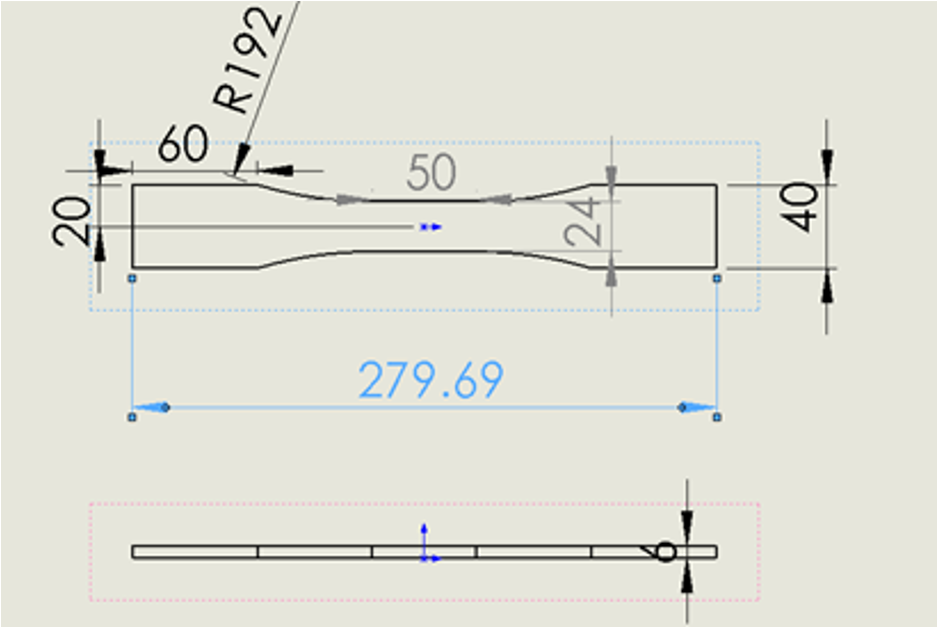
\includegraphics[height=0.7\textwidth]{fig/specimen_dim.png}
%     \caption{Schematic of the 5052-H32 aluminum alloy specimen}
%     \label{fig: specimen dim}
%   \end{subfigure}
%   \begin{subfigure}[t]{0.49\linewidth}
%     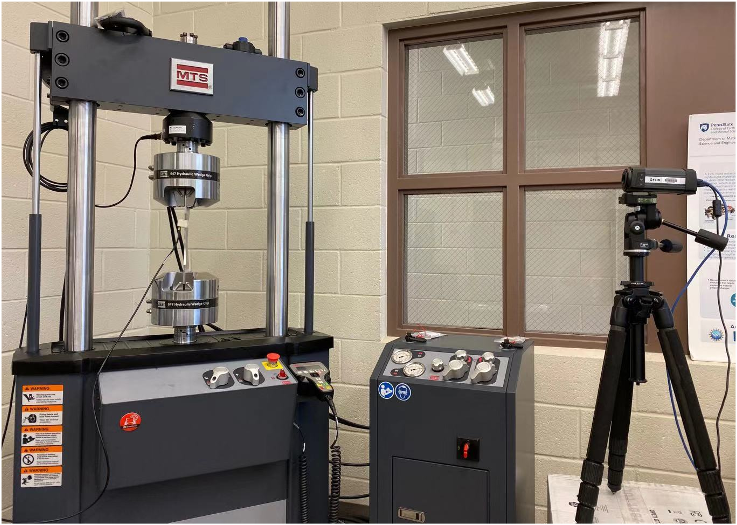
\includegraphics[height=0.7\textwidth]{fig/fatigue_testing_machine.png}
%     \caption{MTS 100KN Landmark fatigue testing system at Prof. Jingjing li's lab}
%     \label{fig: fatigue testing machine}
%   \end{subfigure}

%   \caption{Life cycle fatigue testing setup}
%   \label{fig: fatigue testing setup}
% \end{figure}

% \begin{figure}[tb]
%   \centering
%   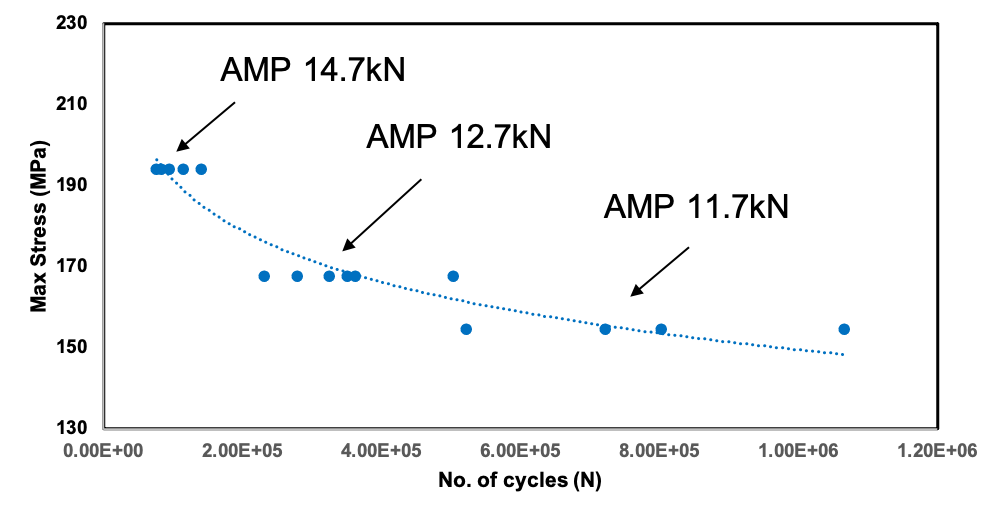
\includegraphics[width=0.8\linewidth]{fig/sn_curve.png}
%   \caption{S-N curve for 5052-H32 aluminum alloy}
%   \label{fig: raw sn curve}
% \end{figure}

\section{Interrupted fatigue testing}
The purpose of performing interrupted fatigue testing is to produce damaged specimens at various fatigue levels by stopping the testing at several predetermined numbers of cycles. Considering the material cost and the time spent, the number of cycles applied to the specimens is set to be two levels, 33\% and 67\% fatigue life corresponding to the three loading amplitudes, 11.7, 12.7, and 14.7 kN. These specimens are used to represent EoL products at different fatigue damage levels from the remanufacturing industry. Besides, three specimens without going through fatigue testing, i.e., 0\% fatigue life, are included as specimens at the healthy state. The summary of the interrupted fatigue testing specimens is presented in Table \ref{table: interrupted specimens}

\begin{table}[tb]
  \centering
  \caption{Summary of the interrupted fatigue testing specimens}
  \label{table: interrupted specimens}
  \begin{tabularx}{0.9\textwidth}{
    >{\centering\arraybackslash}X
    >{\centering\arraybackslash}X
    >{\centering\arraybackslash}X
    >{\centering\arraybackslash}X
  }
    \toprule
    Specimen ID&Loading Amplitude (kN)&Percentage of Fatigue Life (\%)&Max Stress Applied (MPa)\\
    \midrule
    1&11.7&33&176\\
    2&11.7&33&176\\
    3&11.7&67&176\\
    4&11.7&67&176\\
    5&12.7&33&195\\
    6&12.7&33&195\\
    7&12.7&67&195\\
    8&12.7&67&195\\
    9&14.7&33&221\\
    10&14.7&33&221\\
    11&14.7&67&221\\
    12&14.7&67&221\\
    13&--&0&--\\
    14&--&0&--\\
    15&--&0&--\\
    \bottomrule
  \end{tabularx}
\end{table}

\section{Linear and nonlinear ultrasound measurements}
In this research, the LU and NLU testings serve as the two main NDE methods for measuring the accumulated fatigue damage in the specimens. 
% The ultrasonic testing is led by Prof. Matlack's group, and the testing system is shown in Figure \ref{fig: ultrasound setup}. 
The LU and NLU measurements are both 1-D time-domain signals, but the two approaches differ based on different theories and parameters, e.g., excitation wave shape, frequency, and amplitude. Examples of LU and NLU signals are presented in Figure \ref{fig: lu and nlu signals raw}.

The LU and NLU measurements were collected at nine locations on a specimen as illustrated in Figure \ref{fig: measurement locations}, and each location was measured three times to ensure the measurement repeatability. As a result, for each specimen, there are $9 \times 3 = 27$ signal profiles produced. In total, the dataset contains 405 signal profiles.

% \begin{figure}[tb]
%   \centering
%   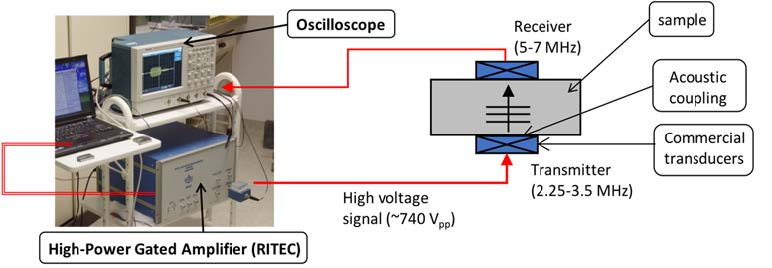
\includegraphics[width=0.9\linewidth]{fig/ultrasound setup.png}
%   \caption{Experimental setup for LU and NLU measurements at Prof. Matlack's Lab}
%   \label{fig: ultrasound setup}
% \end{figure}

\begin{figure}[tb]
  \centering
  \begin{subfigure}[t]{0.49\linewidth}
    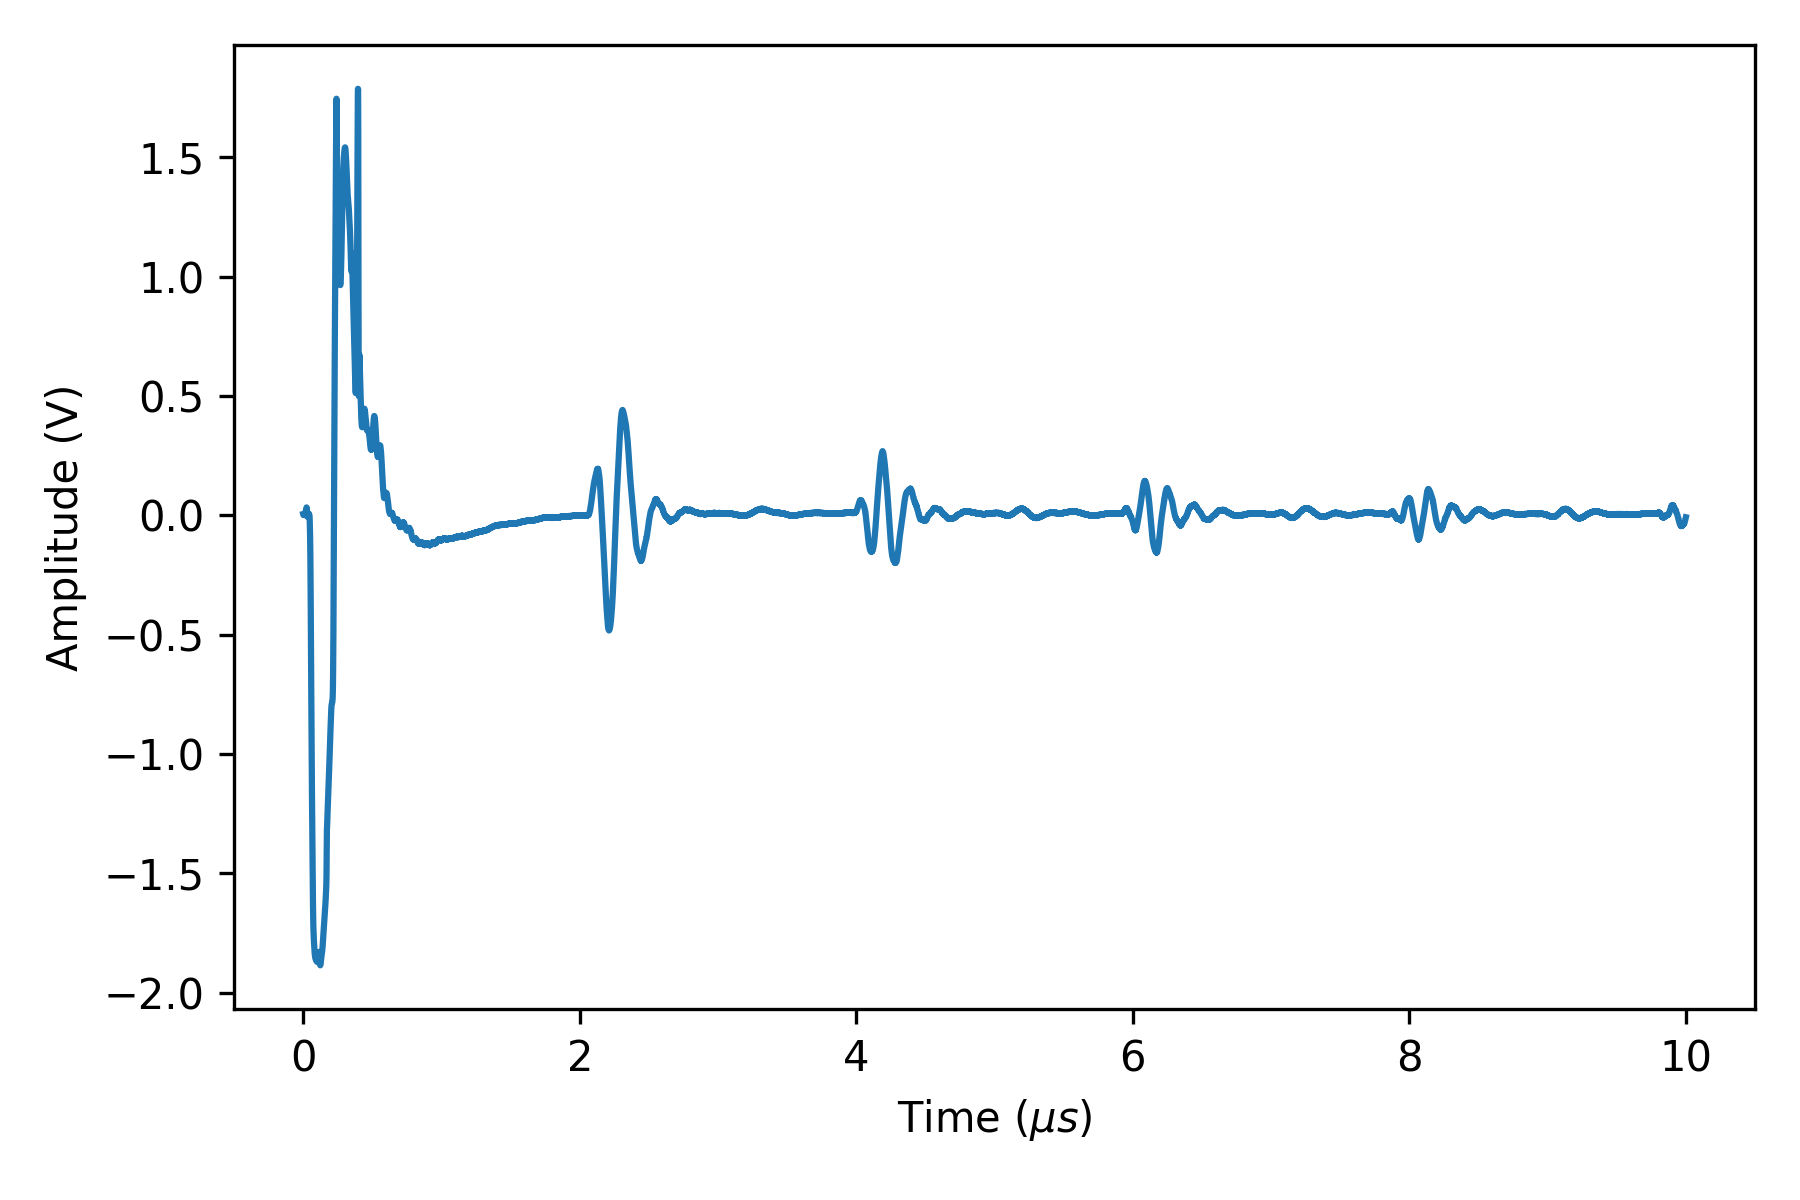
\includegraphics[width=\textwidth]{fig/lu_signal_raw.png}
    \caption{Linear ultrasonic signal}
    \label{fig: lu signal raw}
  \end{subfigure}
  \begin{subfigure}[t]{0.49\linewidth}
    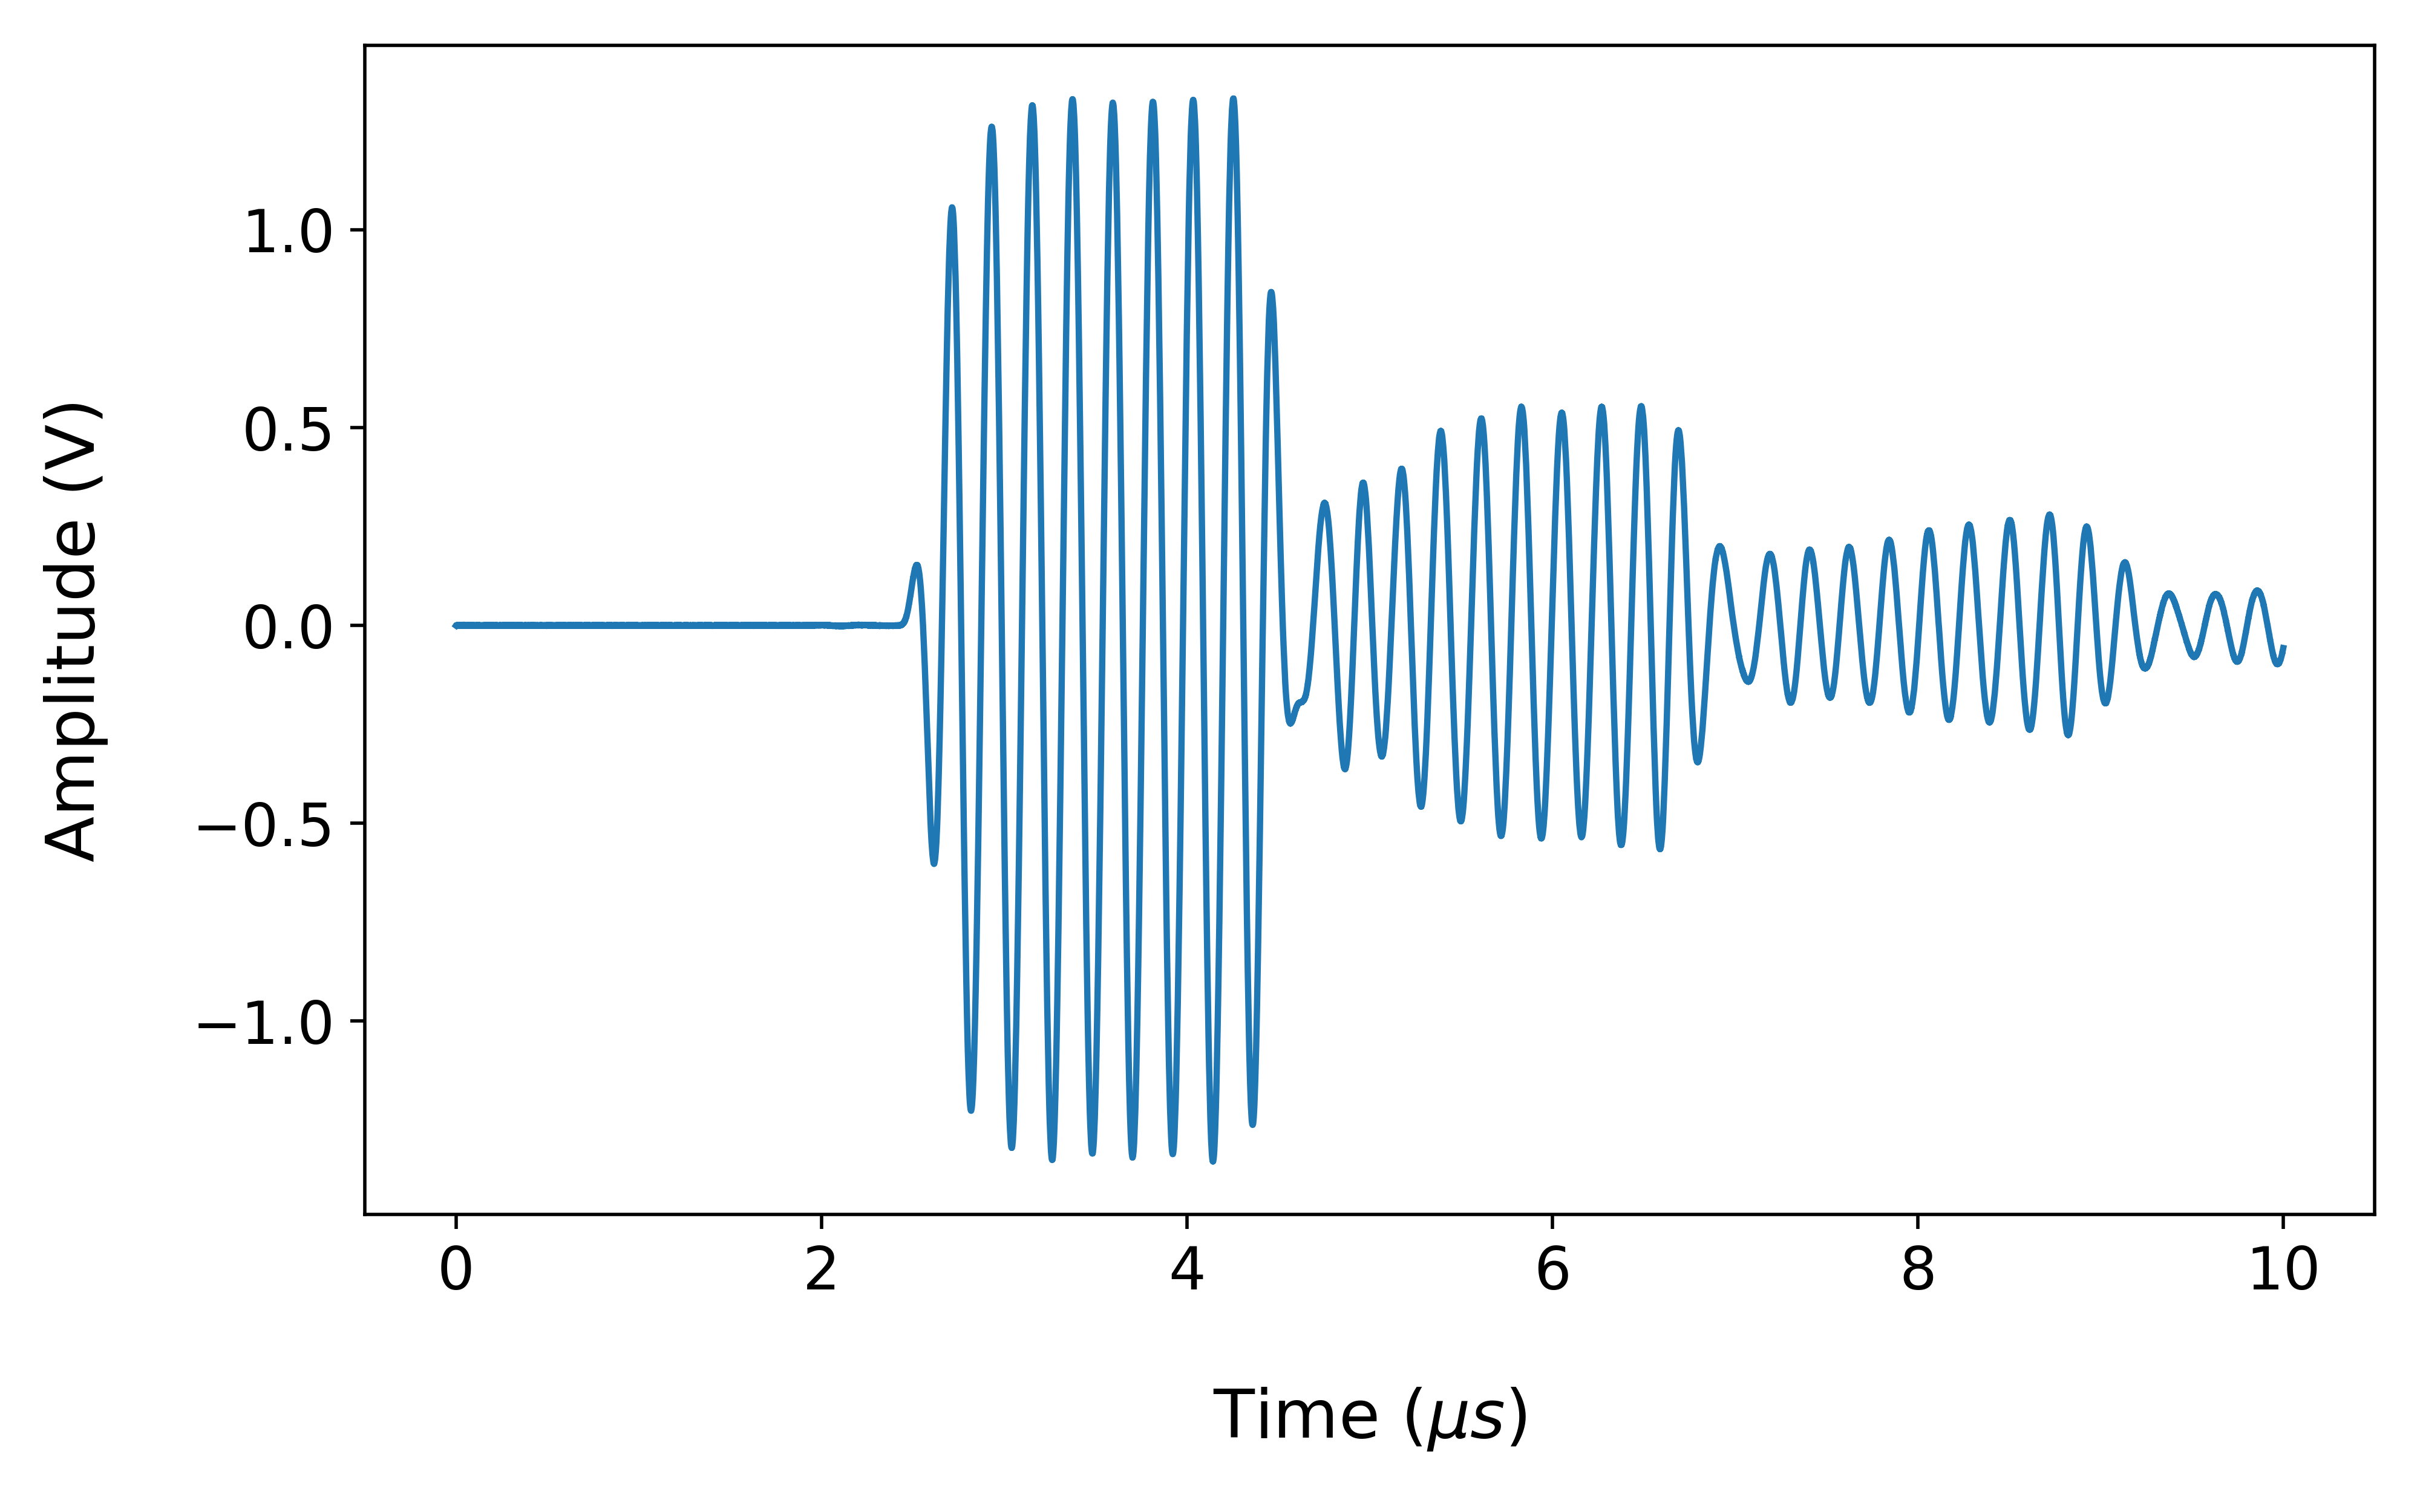
\includegraphics[width=\textwidth]{fig/nlu_singal_raw.png}
    \caption{Nonlinear ultrasonic signal}
    \label{fig: nlu signal raw}
  \end{subfigure}

  \caption{Examples of linear and nonlinear ultrasonic signals}
  \label{fig: lu and nlu signals raw}
\end{figure}

\begin{figure}[tb]
  \centering
  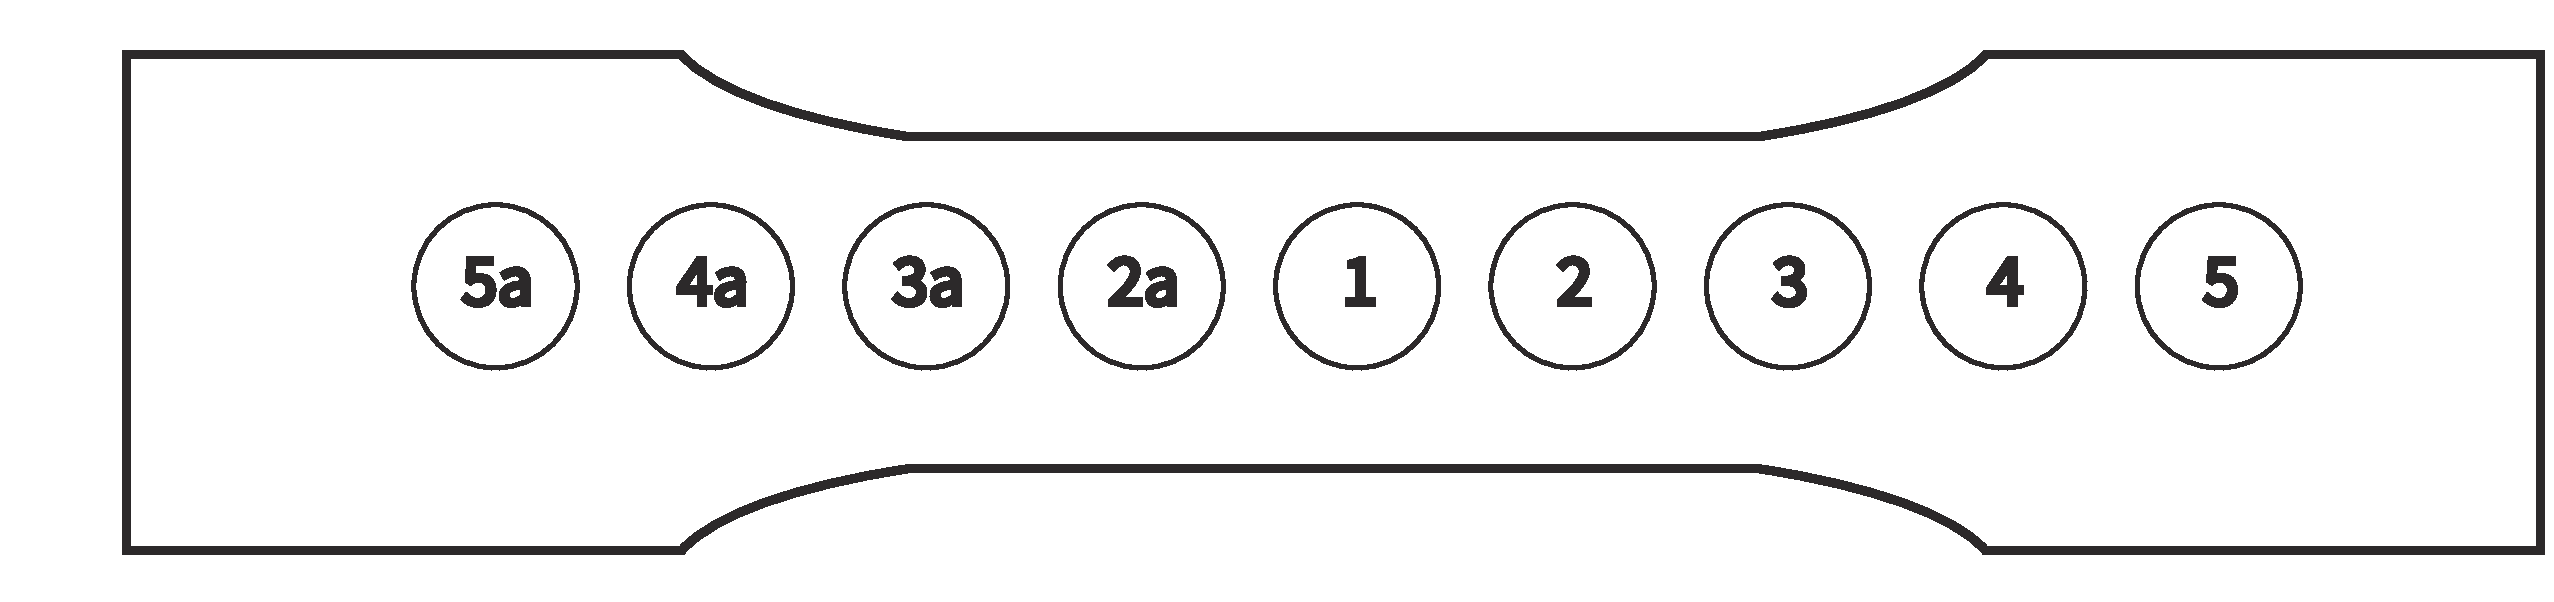
\includegraphics[width=0.6\linewidth]{fig/specimen_measurment_locs.pdf}
  \caption{Schematic of the measurement locations for LU and NLU measurements}
  \label{fig: measurement locations}
\end{figure}

\section{X-ray diffraction measurement}
Another quantity of interest, residual stress, is measured by XRD in this research. Residual stress is known to be associated with fatigue behaviors such as crack initiation and propagation. Besides, the FWHM height of the diffraction peak in XRD is also extracted. The XRD measurements were performed on a subset of the specimens in the interrupted fatigue testing dataset. The residual stress and FWHM measured by XRD are used in the regression tasks in Chapter \ref{chap: reg} as target variables.
